\documentclass[12pt, a4paper]{article}
\usepackage[utf8]{inputenc}
\usepackage{amsmath}
\usepackage{amsthm}
\usepackage{graphicx}
\usepackage{blindtext}
\usepackage{parskip}
\usepackage{hyperref}
\usepackage{graphicx}
\usepackage{url}
\usepackage{listings}
\usepackage{xcolor}
\usepackage{caption}
\graphicspath{ {./images/} }

\title{
  Third Assignment - Validation - SMDE\\
  Juan Pablo Royo Sales\\
  \date\today\vspace{-2em}}
\date{\normalize\today}

\begin{document}

\maketitle

\section{Blackbox Validation}

On the first hand i am running a bunch of experiments according to the DOE
exposed on the previous assignment.

After running the different experiments I got the following results of each
transaction runner that are under \textbf{simulation.csv}.

After doing an \textbf{ANOVA} analysis with the real data of the marathon we
have obtain a very low \textit{p-value} which indicates that the populations are quite
different.

\begin{table}[h!]
  \begin{tabular}{ |c|c|c|c|c|c|c|  }
    \hline
    \multicolumn{7}{|c|}{ANOVA Results from R Studio} \\
    \hline
    & Df & Sum Sq & Mean Sq & F Value & Pr(>F) & \\
    \hline
    x2 & 1 & 38383319841 & 38383319841 & 10458 & $<2e^{16}$ & *** \\
    Residuals & 7198 & 26417268633 & 3670085 & & & \\
    \hline
  \end{tabular}
  \captionof{figure}{ANOVA Analysis between simulation and real marathon data}
  \label{table:anova}
\end{table}

Also we can see the bloxplot resulting on this ANOVA and how the means of both
populations differ, although not so much.

\begin{minipage}[t]{\linewidth}
  \centering
  \includegraphics[width=\textwidth]{plot_comparing_simulation}
  \captionof{figure}{Boxplot ANOVA}
\end{minipage}\\\\

\subsection{Conclusion Blackbox validation}
According to the results we must \textbf{reject the null hypothesis} reaching to
the conclusion that the simulation is not so well adjusted to generate values
near to the real data.

In the context of this Assignment I am not going to adjust the simulation, but
I can assure that if we observe the Plot the means don't diverge so much and
adding more randomness could solve the problem.


\section{Fixed Values}
In fixed values test I have fixed the following values to test the control of
the simulation:

\begin{itemize}
  \item \textbf{KPACE\_M3040} It used to be one of the Distribution Functions in
    the real simulation which indicates in the Linear regression model the pace
    in km 30. I have fixed this to $500$ seconds.
  \item \textbf{IS\_ELITE} Set to $0$ indicating that there is no elite runners
  \item \textbf{WATER\_COIN} Set to $1$ indicating that everyone drink water
  \item \textbf{WC\_COIN} Set to $0$ indicating that no one go to bathroom 
  \item \textbf{SOLID\_COIN} Set to $1$ indicating that everyone take solid food
\end{itemize}

You can check this values in simulation file \textbf{marathon\_boston\_fixed\_values.gps}

According to this values we can predict the following result for each
runner/transaction $F \sim 4505 \text{ seconds}$. It should be almost $5000$ for
seconds for each runner.

How i calculate this number?

Let $P$ be the pace time in each sprint.
Let $S_n$ the number of sprints in the whole race.
Let $W$ be the water amount of waiting time
Let $W_c$ be the number of water points
Let $F$ be the solid food time expend in each solid sport
Let $F_c$ be the amount of solid spots

Therefore, $E[T]$ total expected time would be:

\begin{equation}
  \begin{aligned}
  E[T] &= P*S_n+W*W_c+F*F_c\\
       &= 500*9+1*3+2*1\\
       &= 4505
  \end{aligned}
\end{equation}

\subsection{Results Values}
If I run the simulation with this fixed values we can see how each transaction
arrived at this time as we have stated above. The difference is the $\beta_0$,
$\beta_1$ and $\beta_2$ of my Linear regression model but the previous expected
value is accurate enough as a lower bound of the fixed validation.

\begin{minipage}[t]{\linewidth}
  \centering
  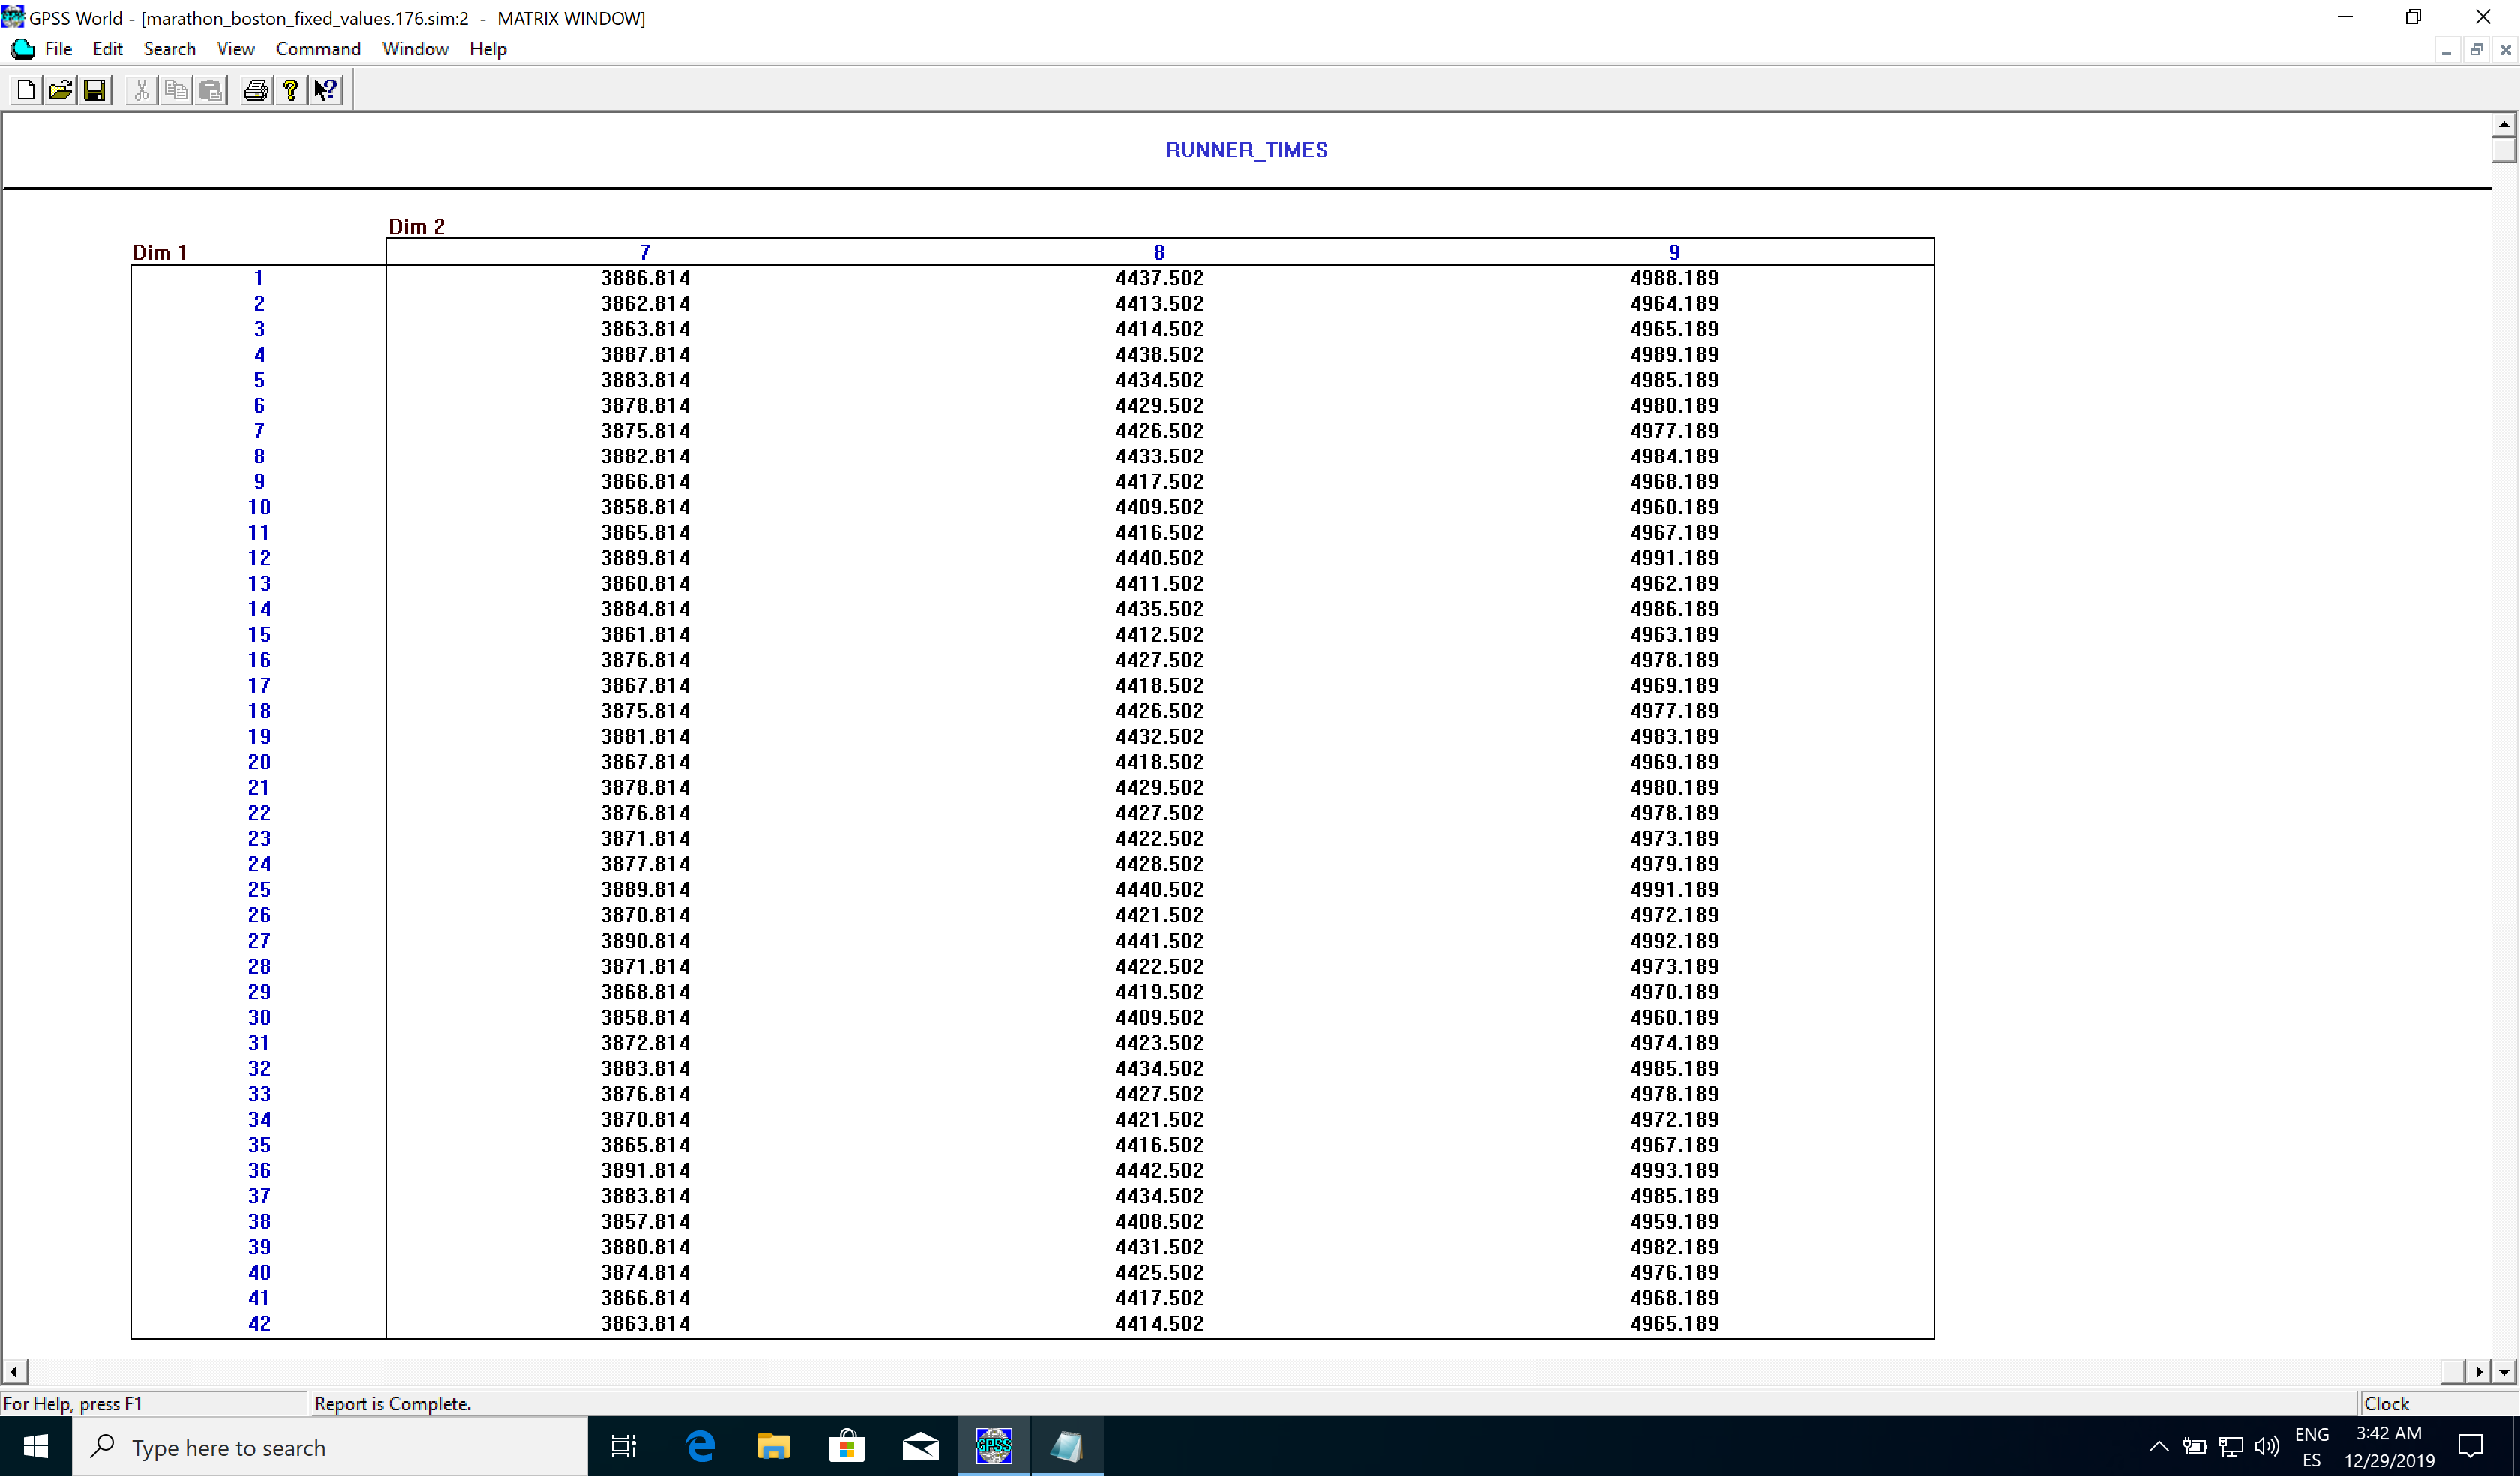
\includegraphics[width=\textwidth]{fixed_values_1}
  \captionof{figure}{Fixed Values Matrix Transaction Results - Sample 1 - Column 9}
\end{minipage}\\\\

\begin{minipage}[t]{\linewidth}
  \centering
  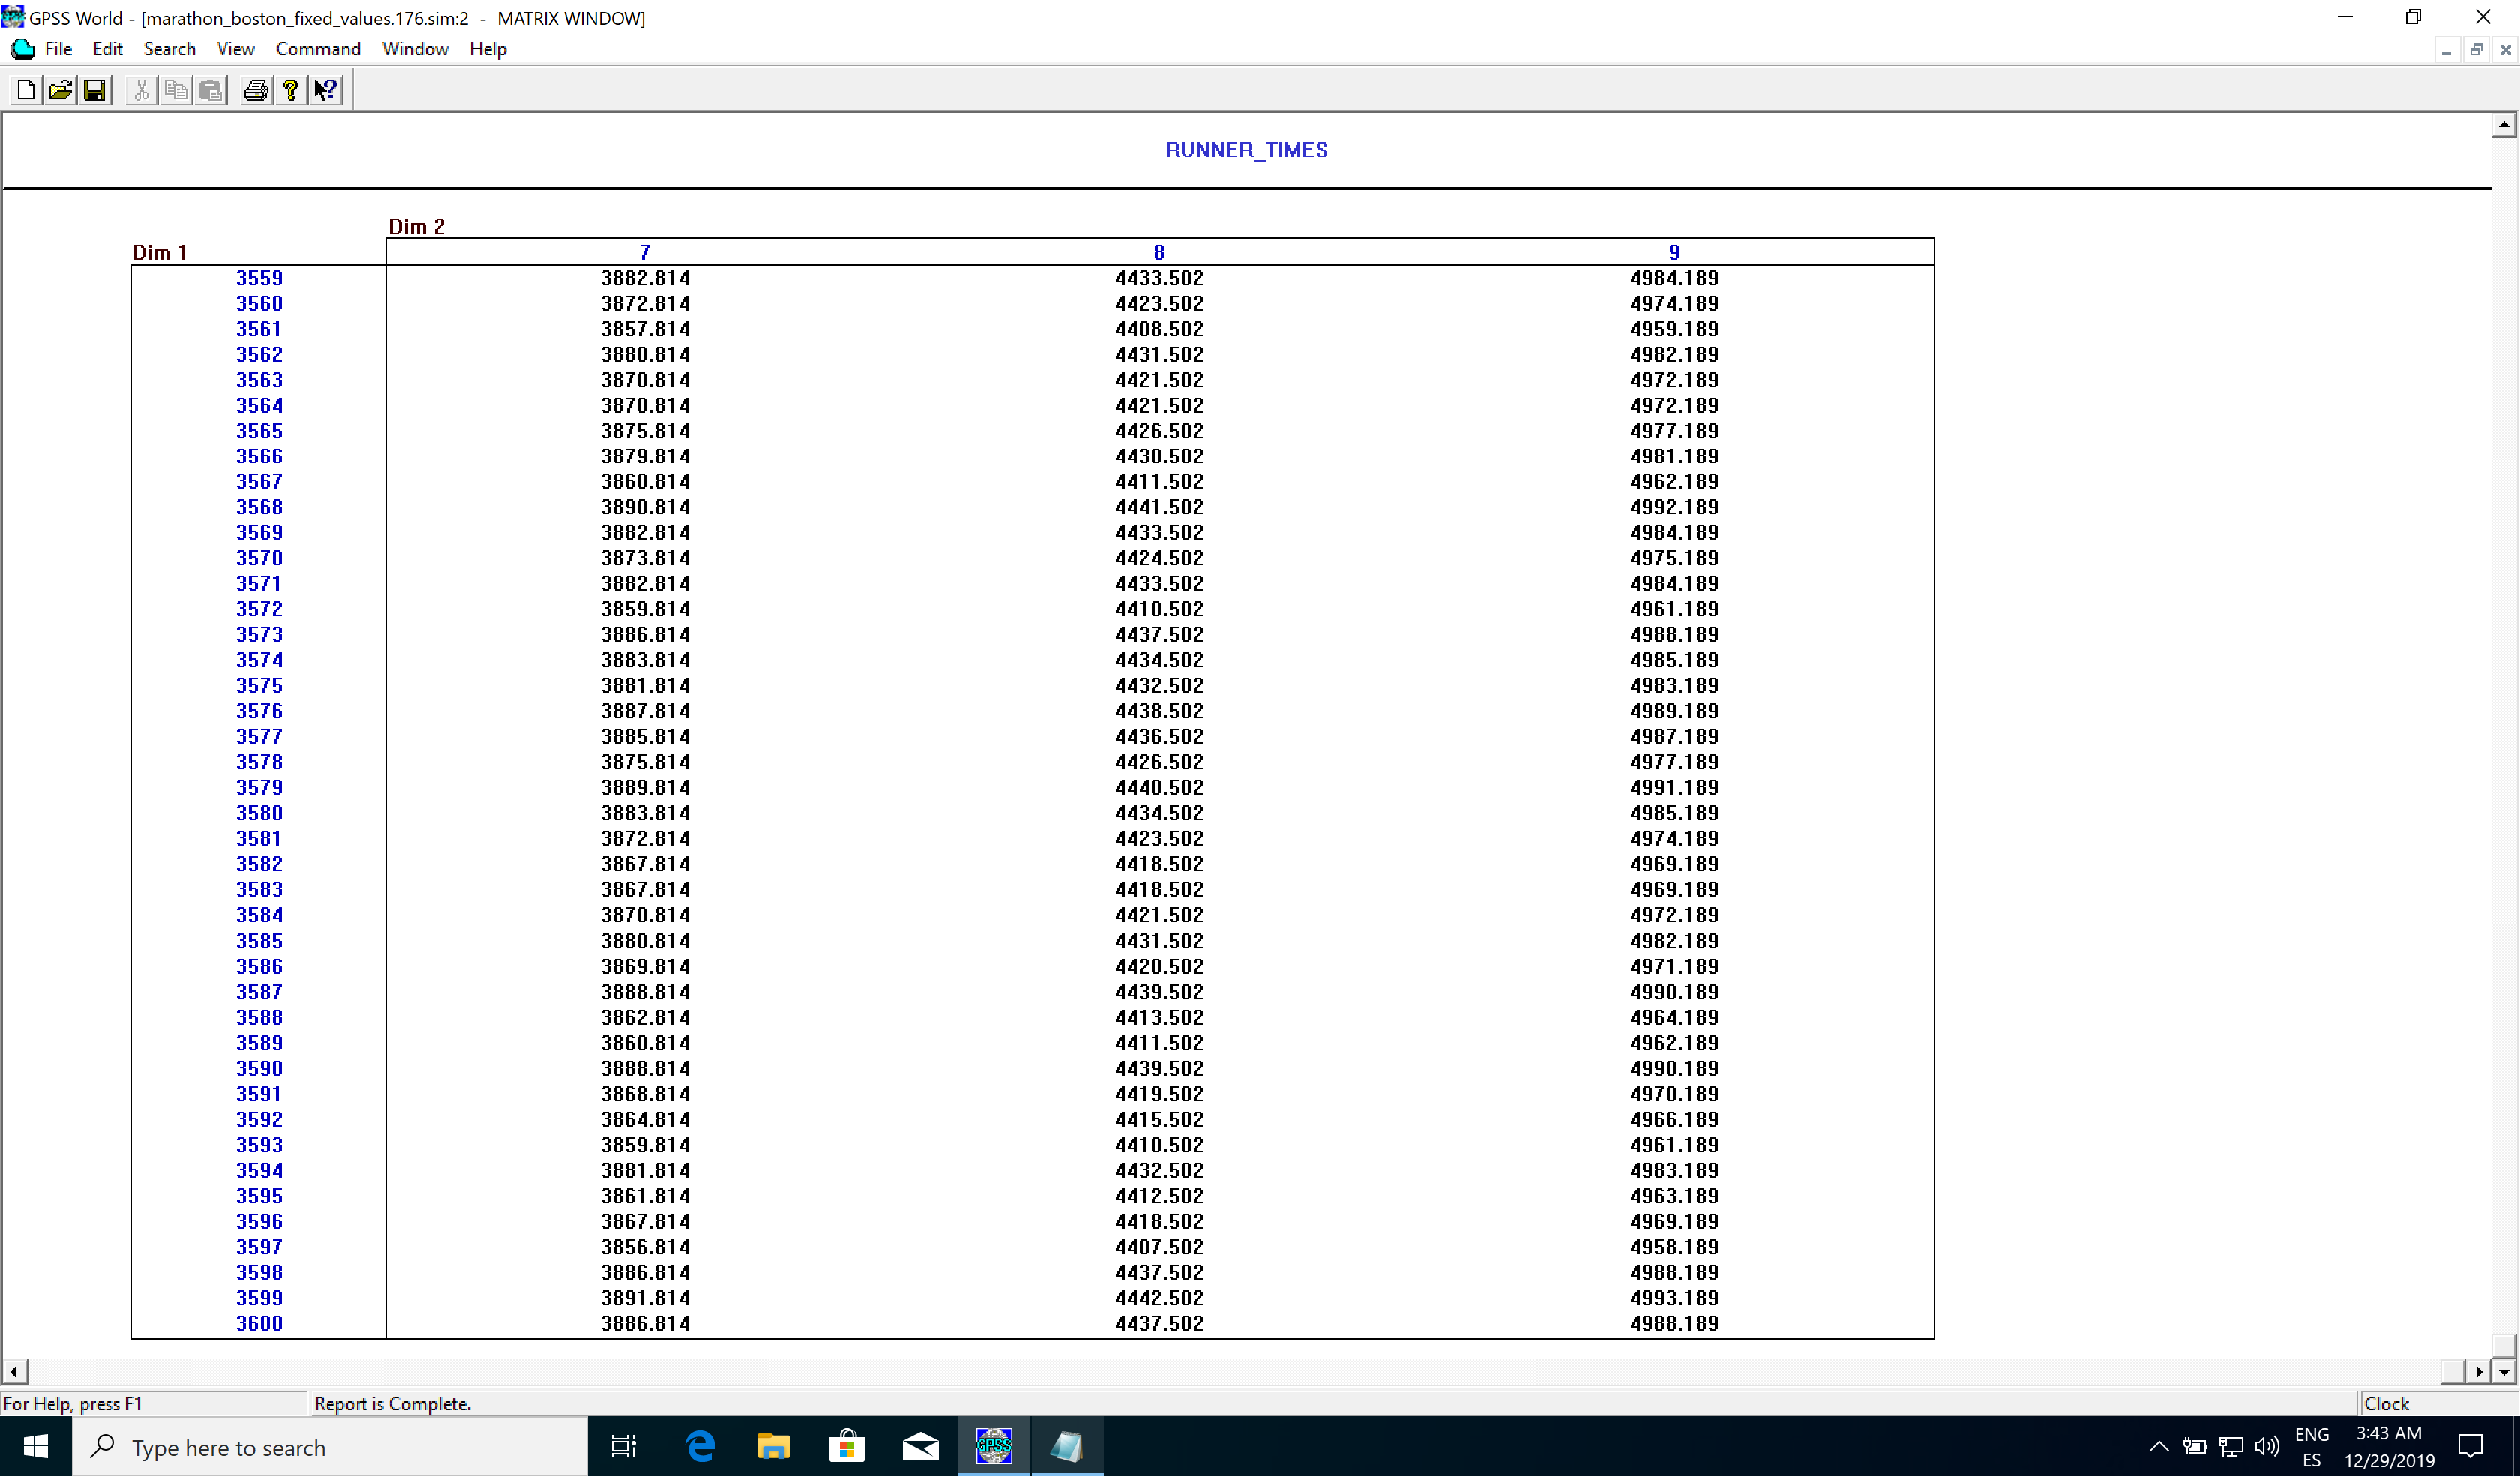
\includegraphics[width=\textwidth]{fixed_values_2}
  \captionof{figure}{Fixed Values Matrix Transaction Results - Sample 2 - Column 9} 
\end{minipage}\\\\

It can also be checked the results of the simulation with fixed values in the
file \textbf{fixed\_values.gpr}


\section{Conclusion}
I believe this has been a great exercise on how to unified all the concepts we
have explored during the subject, since Random Generators, Discrete
Distribution, Normality, ANOVA analysis, Predictions through linear regression
and simulation when multiple agents and factors are involved.

Although the simulation wasn't accurate enough when I validated with the real
data of the marathon, I strongly believe that with a small amount of tuning in
order to simulate more randomness and variability between runners/transactions,
we can reach to a near real simulation with respect to the historical data.



\end{document}
